\chapter{Related Work} \label{chap:Chapter2}       
\epigraph{``This is where technology is now, imagine where we can go in the future” }{\textit{Timothy Chung}}

Σε αυτό το \emph{Chapter} περιγράφονται τρόποι με τους οποί\-ους υπάρχουσες εφαρμογές \Abbr{UAV} swarms, καθώς και 
μεμονωμένων drone - των οποίων οι βασικές αρχές μπορούν να χρησιμοποιηθούν στα σμήνη - επιλύουν το localization pro\-blem. Κάποια από τα συστήματα στις 
παρακάτω έρευνες έχουν καθαρά θεωρητική πλευρά, ενώ, άλλα έχουν δοκιμαστεί σε real-life scenarios.
Τέλος, σε α\-ρκε\-τές από αυτές τις εφαρμογές χρησιμοποιούνται τεχνικές που θα αναλυθούν στο \Chap{Chapter3}
σε μεγαλύτερο βάθος, καθώς θα αποτελέσουν το προαπαιτούμενο θεωρητικό και μαθηματικό υπόβαθρο για τον σχεδιασμό 
του συστήματος της παρούσας διπλωματικής.

Το πρόβλημα του Local Positioning System (\Abbr{LPS}) \cite{lps} έχει ερευνηθεί από διάφορες οπτικές\udot οι 
οποίες μπορεί να βασίζονται σε Radio Frequency (\Abbr{RF}), Sound Waves ή ακόμα και να είναι Optical Oriented.

Σχεδόν βέβαιο είναι επίσης, ότι από όποια κατεύθυνση και αν προσεγγίσουμε το \Abbr{LPS} να έχουμε την ανάγκη να 
χρησιμοποιήσουμε κάποια τεχνική για να συνενώσουμε όλες τις πληροφορίες που έχουμε από τους διάφορους αισθητήρες -
για κάθε μεμονωμένο time-frame - με δεδομένο ότι κάνουμε χρήση πολλαπλών αισθητήρων ώστε να μειώσουμε την εντροπία, 
συνεπώς και την αβεβαιότητα ως προς την εκτίμηση της θέσης. 
Την ανάγκη αυτού έρχεται να καλύψει η έννοια του \emph{sensor fusion} \cite{sensor-fusion}. Όπως επίσης, και την 
ανάγκη φιλτραρίσματος των μετρήσεων - που οδηγεί σε καλύτερα αποτε\-λέ\-σμα\-τα - με μερικούς γνωστούς αλγόριθμους 
που να το επιτυγχάνουν\udot να είναι o Extended Kalman Filter (\Abbr{EKF}), Unscented Kalman Filter (\Abbr{UKF}), 
Covariance Intersection Filter (\Abbr{CIF}),  Split  Covariance  Intersection  Filter (\Abbr{SCIF}) και  Belief  
Propagation (\Abbr{BP}) \cite{fusion-filters}. 

% --------------------------------------------------------------------------------------------------------
% --------------------------------------------------------------------------------------------------------
\section{Radio Frequency}
Το πιο εύκολο που μπορούμε να φανταστούμε είναι να χρησιμοποιήσουμε \Abbr{RF} τε\-χνο\-λο\-γίες όπως \Abbr{GPS}, WiFi, Zigbee, Bluetooth, Ultra-Wideband (\Abbr{UWB}) ή ακόμα και άλλα\udot για την επικοινωνία και την υλοποίηση του \Abbr{LPS}. Συχνός παράγοντας για το ποιο θα επιλεχθεί, σχετίζεται αν η εφαρμογή μας κυμαίνεται σε short ή long range εμβέλειες.

Άλλοι παράγοντες, ως παράδειγμα, είναι ότι το WiFi είναι εύκολα προσβάσιμο\udot με μικρό κόστος, ενώ το Zigbee προτιμάται για low power consumption εφαρμογές. Όμως προβλήματα, μπορεί να είναι, ότι στο WiFi είναι πολύ εύκολο να υπάρχουν παρεμβολές από τις υπόλοιπες γειτονικές 
συσκευές\footnote{Αυτό μπορεί να είναι αρνητικό για κάποιες εφαρμογές σε indoor scenarios} 
άρα δεν το καθιστά καλή λύση για κάθε αποστολή ενός swarm. Το Zigbee επιλύει γενικά κάποιες από τις αδυναμίες του WiFi\footnote{Σε indoor σενάρια παραμένει η δυσκολία για collision-free formation} όμως ταυτόχρονα πρέπει να αποδεχτούμε το μικρό data rate που μπορούμε να μεταδώσουμε. 
Συχνή εφαρμογή έχουν επίσης τα \Abbr{UWB} καθώς επιλύουν θέματα σχετικά με την ακρίβεια των μετρήσεων, 
το κόστος καθώς και την εμβέλεια\udot ταυτόχρονα \cite{uwb-imu-gps3}. 

Τέλος, θετικό στην χρήση \Abbr{RF} τεχνολογιών, είναι αρχικά ότι δεν χρειαζόμαστε άμεση οπτική επαφή με το ιπτάμενο, ενώ επίσης ότι μπορούμε εύκολα να δημιουργήσουμε
ένα Flying Ad-hoc Network (\Abbr{FANET}) το οποίο βοηθάει στην ευελιξία του συστήματος.

% --------------------------------------------------------------------------------------------------------
% --------------------------------------------------------------------------------------------------------
\subsection{WiFi}
Μία αρχική προσέγγιση για τον εντοπισμό ενός drone δίνεται από τους συγγραφείς του \cite{wifi-passive-active-drone-localization}
οι οποίοι χρησιμοποιούν WiFi προκειμένου να εντοπίσουν την θέση του αεροχήματος. Το ενδιαφέρον - με την χρήση του WiFi - είναι ότι, 
είναι μία εύκολη λύση όταν αναφερόμαστε για short range localization. 

Ο τρόπος με τον οποίο προσεγγίζουν το πρόβλημα, είναι με 
το να προσπαθήσουν να αξιοποιήσουν - από την πλευρά του WiFi based - τις τεχνικές, 
Passive Bistatic Radar (\Abbr{PBR}) και Passive Source Location (\Abbr{PSL}), να χρησιμοποιήσουν Kalman Filter (\Abbr{KF})
και τέλος να πραγματοποιήσουν Data Fusion τεχνικές στους δύο αισθητήρες που χρησιμοποιήθηκαν\udot ώστε να γίνει ο εντοπισμός της θέσης.

Ξεκινώντας με τη τεχνική \Abbr{PBR}, η οποία αξιοποιεί τα echoes που
γίνονται scatter από τα εμπόδια που υπάρχουν στον χώρο\udot προκειμένου να εντοπίσει το αντικείμενο. Έχει σαν κύρια χαρακτηριστικά 
ότι χρησιμοποιείται για εντοπισμό κινούμενων α\-ντι\-κειμένων και δεν χρειάζεται το ίδιο το αντικείμενο να εκπέμπει σήματα, πράγμα που 
το καθιστά ιδανικό για εντοπισμό non-cooperative στόχων. Προκειμένου βέβαια να εκτιμηθεί η θέση, έπειτα από την αρχική επεξεργασία 
που γίνεται από τα λαμβανόμενα echoes, ο εντοπισμός τελικά της θέσης πραγματοποιείται μέσω ενός συνδυασμού από μετρήσεις με βάση 
range είτε γωνία. 

Αντίθετα, με την τεχνική \Abbr{PSL} - η οποία προαπαιτεί stationary αντικείμενα - είναι σημαντικό να λαμβάνουμε πακέτα από το 
αντικείμενο ενδιαφέροντος, καθώς εκτιμάει την θέση του\udot μέσω των πακέτων που λαμβάνει, σε συνδυασμό με μία μέτρηση \Abbr{AoA} 
και μία \Abbr{TDoA} (στο \Sect{Energy-based} γίνεται ανάλυση τους).

Συνοπτικά οι συγγραφείς της συγκεκριμένης έρευνας, παρουσιάζουν στο \Fig{PBR-and-PSL} (a) τον γενικό τρόπο λειτουργίας των δύο 
μεθόδων, ενώ στο \Fig{PBR-and-PSL} (b) τις διαφορές τους.

% IMAGE
\begin{figure} [H]
	\centering
    % -----------------
		\begin{minipage}{.47\textwidth}
			\centering
			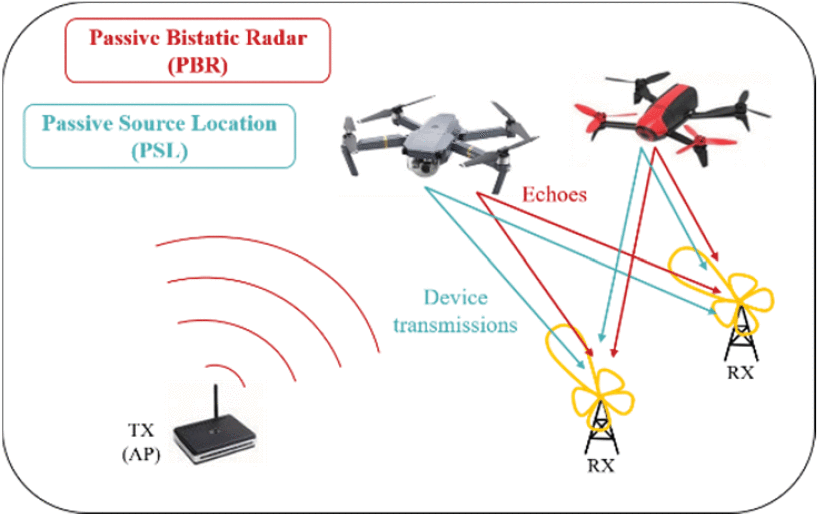
\includegraphics[width=.9\linewidth]{Images/Related-Work/PBR-and-PSL-approaches.png}\\
			{(a) PBR and PSL \URI{https://ieeexplore.ieee.org/document/9253794/figures}}
		\end{minipage}%
		\hspace*{+0.8cm}
		% -----------------
		\begin{minipage}{.47\textwidth}
			\centering
			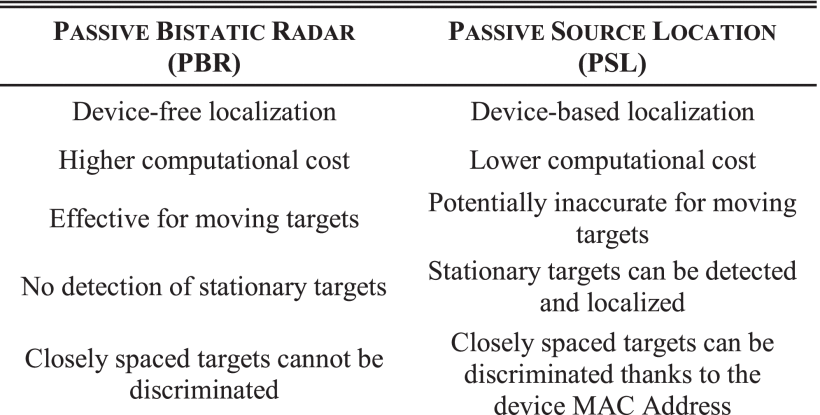
\includegraphics[width=.9\linewidth]{Images/Related-Work/PBR-and-PSL-Features.png}\\
			{(b) PBR and PSL Features \URI{https://ieeexplore.ieee.org/document/9253794/figures}}
		\end{minipage}
	% -----------------
    \hfill \break
    \decoRule
    \caption[PBR and PSL localization Approaches]{PBR and PSL localization Approaches based on \cite{wifi-passive-active-drone-localization}}
    \label{fig:PBR-and-PSL}
\end{figure}

Για την υλοποίηση χρησιμοποιήθηκε ένα DJI Mavic Pro, το οποίο ήταν το drone του οποίου η θέση έγινε προσπάθεια να εκτιμηθεί.
Σχετικά με το σκέλος του \Abbr{PBR} χρησιμοποιήθηκε ένα Access Point (AP, D-Link DAP1160), το οποίο ήταν συ\-νδε\-δε\-μέ\-νο 
σε μία transmitting directive antenna (TP-LINK TL-ANT2409A). Ενώ για τα receivers χρησιμοποιήθηκαν οι ίδιες κεραίες σε συνδυασμό 
με ένα URSP-2955 της National Instruments.

% --------------------------------------------------------------------------------------------------------
% --------------------------------------------------------------------------------------------------------
\subsection{UWB}
Όπως αναφέρθηκε στην αρχή αυτού του κεφαλαίου, ένας τρόπος προσδιορισμού της θέσης\udot είναι με χρήση \Abbr{UWB}.
Ένα από τα πλεονεκτήματα της χρήσης \Abbr{UWB} είναι η ικανότητα υπολογισμού της σχετικής απόστασης μεταξύ δύο
σημείων με σφάλμα απόκλισης μικρότερο των 0.1m \cite{uwb-accuracy}.

Συγκεκριμένα, οι συγγραφείς του \cite{uwb-imu-gps1} πραγματοποιούν Sensor Fusion, βασισμένα σε μετρήσεις 
\Abbr{GPS}/\Abbr{IMU}/\Abbr{UWB} προκειμένου να εκτιμήσουν την θέση 
7 Fixed-Wing \Abbr{UAV}<s> σε εξωτερικό χώρο.

Ο τρόπος με τον οποίο το επιτυγχάνουν, συνοπτικά, είναι ο εξής. Κάθε drone είναι σε θέση να συλλέξει για τον εαυτό του 
- μέσω των αισθητήρων - πληροφορίες όπως τις συντεταγμένες του, το διανύσματα της ταχύτητας του, της
επιτάχυνσης του και τέλος μέσω \Abbr{UWB}\udot και χρήση μίας τεχνικής που ονομάζεται Single-sided Two-way Ranging 
(\Abbr{SS-TWR}) - ουσιαστικά μία \Abbr{ToA}-based προσέγγιση (η οποία γενικά αναφέρεται 
στο \Sect{Distance-Angle-Estimation}) - να υπολογίσει την απόσταση που βρίσκεται σε σχέση με κάθε γειτονικό ιπτάμενο.

Αφού συλλεχθούν οι παραπάνω πληροφορίες, γίνεται το απαραίτητο preprocessing, το οποίο περιλαμβάνει την πραγματοποίηση μετασχηματισμών
και φιλτραρίσματος με χρήση \Abbr{EKF}, ώστε να δημιουργηθεί μία καλύτερη εκτίμηση της κάθε απόστασης με τα γειτονικά drones.

Στην συγκεκριμένη έρευνα, μοντελοποιούν το σύστημα ως ένα time-varying undirected γράφο τον οποίο τον διαχειρίζονται ως ένα spring system - 
όπως παρουσιάζεται στο \Fig{spring-system} - με διαφορετικούς συντελεστές σκληρότητας και προσπαθούν να βρουν το σημείο ισορροπίας του, 
που τελικά είναι το σημείο με την ελάχιστη συνολική δυναμική ενέργεια. Ουσιαστικά μετατρέπουν το position estimation problem σε ένα 
non-convex optimization problem.

% IMAGE
\FigCaptLabelBasedURL{Images/Related-Work/paper-spring.png}
{An illustration of the spring system}%
{spring-system}%
<0.45>%
[uwb-imu-gps1]%
(https://www.researchgate.net/publication/345459052_Cooperative_3-D_relative_localization_for_UAV_swarm_by_fusing_UWB_with_IMU_and_GPS)

Σχετικά με το υλικό που χρησιμοποιήθηκε, έγινε χρήση ενός NEO-M8N \Abbr{GPS} της U-blox με συχνότητα ανανέωσης τα 5Hz.  
Σε κάθε \Abbr{UAV} χρησιμοποιήθηκε ένα Pixhawk PX4 flight management unit. Για το κομμάτι του \Abbr{UWB} έγινε χρήση
ενός module LinkTrack, για την επικοινωνία με το ground station χρησιμοποιήθηκε ένα UBNT, ενώ η επεξεργασία των 
αλγορίθμων έγιναν σε ένα Raspberry Pi 3B+. 

Τέλος, τα αποτελέσματα που κατάφεραν να έχουν ήταν, \Abbr{3D} relative position estimation με σφάλμα απόκλισης τα 0.4m. 

% --------------------------------------------------------------------------------------------------------
% --------------------------------------------------------------------------------------------------------
\subsection{Cellular Networks}
Ένας ακόμα εφικτός τρόπος προσέγγισης - για την εκτίμηση της θέσης - είναι με χρήση
cellular networks. Η εξέλιξη των mobile networks (GSM/LTE/5G) έχει οδηγήσει να γίνουν προσπάθειες εκτίμησης
της θέσης των drones με την βοήθεια αυτών των τεχνολογιών, παράδειγμα της μεθόδου βρίσκεται στο \Fig{cellular-network}. 

% IMAGE
\FigCaptLabelBasedURL{Images/Related-Work/cellular.png}
{Cellular network}%
{cellular-network}%
<0.5>%
[cellular-network-localization]%
(https://ieeexplore.ieee.org/abstract/document/9120588/figures)

Συγκεκριμένα, οι συγγραφείς του \cite{cellular-network-localization} ερευνούν από την θεωρητική οπτική το συ\-γκε\-κρι\-μένο πρόβλημα, 
και αφού το μοντελοποιήσουν\udot χρησιμοποιούν Monte Carlo simulation και το snapshot model, προκειμένου να αναλύσουν την επιρροή 
των διάφορων παραμέτρων του συστήματος στην τελική απόδοση διάφορων localization τεχνικών (όπως με χρήση \Abbr{TDoA}). Τέτοιοι 
παράμετροι - που υπάρχουν σε αυτά τα δίκτυα - είναι το πλήθος των κεραιών με τις οποίες μπορούμε να επικοινωνήσουμε και το πόσο συγχρονισμένες 
είναι, τα χαρακτηριστικά του air-to-ground καναλιού καθώς και το αν υπάρχει ενδιάμεση ύπαρξη εμποδίων σε καθένα από αυτά. Όπως, και το 
ύψος του αεροχήματος σε συνδυασμό με τις λαμβανόμενες παρεμβολές.

% --------------------------------------------------------------------------------------------------------
% --------------------------------------------------------------------------------------------------------
\subsection{Lora}

Ο τομέας των Internet of Things (\Abbr{IoT}) έχει επιφέρει στην έντονη χρήση\udot για πολλές τεχνολογίες, με τα Long Range Wide Area Network (\Abbr{LoRaWAN}) - που πρακτικά αποτελούν παρακλάδι του ευρύτερου τομέα των Low Power Wide Area Network (\Abbr{LPWAN}) - να είναι μία από αυτές. Λόγοι που χρησιμοποιούνται συχνά - για τέτοιες εφαρμογές - είναι ότι τα Low Power Networks (\Abbr{LPN}) είναι ιδανικά όταν μας ε\-νδια\-φέ\-ρει το 
power consumption ενός συστήματος, καθώς επίσης και η μεγάλη εμβέλεια των \Abbr{LoRaWAN}, που μπορούν να φτάσουν σε ακτίνες επικοινωνίας ακόμα και 2km σε κατοικημένες περιοχές εξυπηρετώντας χιλιάδες κόμβους σε ένα σύστημα \cite{lora-localization}.

Οι συγγραφείς του \cite{lora-localization} αξιοποιούν τα πλεονεκτήματα αυτά,
και τα χρησιμοποιούν - παρόλο που δεν είναι σχεδιασμένα για αυτό το λόγο - επεκτείνοντας ένα σύστημα από στατικούς κόμβους, σε ένα και με δυναμικές μετρήσεις\udot με την βοήθεια drone σαν \Abbr{3D} mobile gateway stations - \Fig{lora-system-setup}, όπου καταφέρνουν να βελτιώσουν έως και 10 φορές την ακρίβεια εκτίμησης της θέσης ενός αντικειμένου.

% IMAGE
\FigCaptLabelBasedURL{Images/Related-Work/lora-system-setup.png}%
{Lora system setup}%
{lora-system-setup}%
<0.55>%
[lora-localization](https://www.researchgate.net/figure/System-setup_fig1_341344946)

Για να το καταφέρουν, αξιοποιούν πληροφορία σχετικά με την ένταση της ισχύς των λαμβανόμενων πακέτων, μοντελοποιούν αυτήν την σχέση για να καταφέρουν να εκτιμήσουν την απόσταση μεταξύ δύο κόμβων και στην συνέχεια με χρήση αυτών των αποστάσεων, καταφέρνουν να 
βρουν την θέση του αντικειμένου (στο \Chap{Chapter3} υπάρχει ανάλυση των μεθόδων που ακολουθήθηκαν).

Η έρευνα τους περιστρέφεται στο develop και testing ενός search algorithm, τόσο από την πλευρά των simulation καθώς και ως real system, καταλήγοντας σε διάφορα συμπεράσματα - με βάση την χρήση διαφορετικού πλήθος drone σε συνδυασμό με διαφορετικών συχνοτήτων λήψεις μετρήσεων.

Σχετικά με τις τεχνολογίες που χρησιμοποιήθηκαν, ο search αλγόριθμος αρχικά δοκιμάστηκε σε 
MATLAB simulations ενώ στην συνέχεια σε Software In The Loop (\Abbr{SITL}) simulations χρησιμοποιώντας 
το Gazebo. Τέλος, στο κομμάτι του hardware, το κάθε drone ήταν εξοπλισμένο με ένα PixHawk flight το οποίο έτρεχε PX4 autopilot, ένα Raspberry Pi 3B+ στο οποίο υπήρχε το Robot Operating System (\Abbr{ROS}) και το MAVROS, ένα MultiTech MultiConnect Conduit LoRa gateway και η σύνδεση στο Swisscom \Abbr{LoRaWAN} έγινε με την βοήθεια ενός Huawei E3372 USB modem.

% --------------------------------------------------------------------------------------------------------
% --------------------------------------------------------------------------------------------------------
\subsection{RTK GNSS}
Ένας εύκολα προσβάσιμος τρόπος - για την εκτίμηση θέσης αντικειμένου - που ο καθένας εύκολα μπορεί να χρησιμοποιήσει, σχετίζεται με τους δορυφόρους και τη χρήση \Abbr{GNSS} τεχνικών όπως το \Abbr{GPS}.

Παρόλο, την πολλά υποσχόμενη, εξέλιξη της ακρίβειας από $\sim$5m \cite{gps-accuracy}
σε $\sim$30cm \cite{superaccurate-gps} - για μη στρατιωτική χρήση -
η οποία όμως επίσης δεν είναι αρκετή για τις ανάγκες ορισμένων εφαρμογών. 
Πολλές φορές οδηγούμαστε να κινηθούμε σε αρκετά ακριβές 
λύσεις διορθώσεις των σφαλμάτων, και να χρησιμοποιήσουμε  Real Time Kinematic (\Abbr{RTK}) \cite{rtk-gps} τεχνικές, οι οποίες είναι ικανές να προσφέρουν ακρίβεια 1-2cm σε ακτίνες $\sim$20km. 

% IMAGE
\FigCaptLabelBasedURL{../Photos/RTK.png}%
{RTK usage Principle}%
{rtk-usage}%
<0.42>%

Η γενική αρχή λειτουργίας του \Abbr{RTK}-\Abbr{GPS}, είναι ότι αποτελείται από ένα επίγειο
base station - ουσιαστικά μιλάμε για μία stationary \Abbr{GPS} master antenna - του οποίου οι
συντεταγμένες είναι γνωστές εξ' αρχής. Αυτός είναι υπεύθυνος να συ\-γκρί\-νει τα carrier phase των λαμβανόμενων σημάτων από τους δορυφόρους\udot προκειμένου να κάνει τις απαραίτητες διορθώσεις, τις
οποίες αποστέλλει στην συνέχεια - μέσω του πρωτοκόλλου Radio Technical Commission for Maritime Service
(\Abbr{RTCM}) - στα κινούμενα rover, τα οποία τελικά επιθυμούν να υπολογίσουν την θέση τους. Απλοποιημένο παράδειγμα αυτού, βρίσκεται στο \Fig{rtk-usage}.

Οι συγγραφείς του \cite{rtk-gps-drone-localization} πραγματοποιούν μεγαλύτερη ανάλυση λει\-του\-ργίας του, α\-να\-φέ\-ρουν λόγους ύπαρξης προβλημάτων, καθώς προτείνουν και μία αρχιτεκτονική η οποία μπορεί να βελτιώσει το availability του \Abbr{RTK}-\Abbr{GPS} σε ένα multi-vehicle system.

% --------------------------------------------------------------------------------------------------------
% --------------------------------------------------------------------------------------------------------
\section{Sound Waves} \label{sec:related-sound}
Μία εναλλακτική εκδοχή προσέγγισης υπολογισμού της θέσης, είναι με την βοήθεια ακουστικών κυμάτων. Παρόλο που αναλογικά με τις άλλες μεθόδους δεν είναι τόσο συχνά χρησιμοποιούμενη, υφίσταται ερευνητικό ενδιαφέρον για προσπάθειας α\-πό\-κτη\-σης location information με χρήση ήχου. 

Υπάρχουν εφαρμογές στις οποίες χρειάζεται να ανιχνευτεί η θέση non cooperative - ακόμα και εχθρικών - drone τα οποία είτε να μην μπορούν να ανιχνευτούν - λόγο μεγέθους - από κάμερα είτε να μην μπορεί να χρησιμοποιηθεί κάποια \Abbr{RF} τεχνική.
Στην έ\-ρ\-ευ\-να \cite{sound-waves-for-drone-localization} οι συγγραφείς εμπνευσμένοι από αυτό, κάνουν προσπάθεια δημιουργίας ενός συστήματος παρακολούθησης, για localization και tracking ενός drone με την χρήση acoustic arrays - παρουσιάζονται στο \Fig{acoustic-arrays}. 

% IMAGE
\FigCaptLabelBasedURL{Images/Related-Work/acoustic-arrays.png}%
{Acoustic Arrays for localization}%
{acoustic-arrays}%
<0.55>%
[sound-waves-for-drone-localization]%
(https://ieeexplore.ieee.org/document/8448409/figures)

Συγκεκριμένα, τοποθετούν σε συγκεκριμένες θέσεις τα δύο arrays, από τα οποία λα\-μβά\-νουν, με χρήση Generalized Cross Correlation - Phase Transform (\Abbr{GCC-PHAT}), ένα πλήθος μετρήσεων \Abbr{TDoA} μεταξύ των δύο arrays. Λόγο όμως το ότι από μόνες τους αυτές οι
μετρήσεις - εξ' αιτίας του multipath effect - καταλήγουν να περιλαμβάνουν σφάλματα, προτείνουν έναν βασισμένο στο Gauss
priori Probability Density Function (\Abbr{GPDF}) αλγόριθμο\udot ώστε τελικά να εντοπίσουν την θέση των drone, ενώ στην συνέχεια χρησιμοποιούν \Abbr{KF} για να το κάνουν track.

Ο εξοπλισμός που χρησιμοποιήθηκε ήταν sensors τύπου CHZ-213 1/2-inch me\-tro\-lo\-gi\-cal microphones, με κάθε sensor εφοδιασμένο με ένα pre-amplifiers τύπου YG-201. Ενώ, το drone του οποίου έγινε προσπάθεια να εκτιμηθεί η θέση ήταν το DJI Pha\-ntom 2. Τα αποτελέσματα που είχαν, ήταν να καταφέρουν στο μεγαλύτερο ποσοστό των εκτιμήσεων, τα σφάλματα να είναι μικρότερα των 6m σε μέγιστη απόσταση κάλυψης τα 100m.  

% --------------------------------------------------------------------------------------------------------
% --------------------------------------------------------------------------------------------------------
\section{Optical Oriented} \label{sec:related-optical}
Το πρόβλημα της εκτίμησης θέσης ενός αντικειμένου, έχει επίσης επιστημονικό ε\-νδια\-φέ\-ρον να λυθεί με χρήση οπτικών μέσων. Τέτοιοι τρόποι μπορεί να είναι με χρήση mo\-no\-cu\-lar κάμερας, stereo κάμερας ή τεχνικές που σχετίζονται με το φως - με μερικές από αυτές, να αναλύονται συνοπτικά στην συνέχεια του κεφαλαίου.

% ---------------------------------------------------------------------------------------------------------
% ---------------------------------------------------------------------------------------------------------
\subsection{Camera} \label{sec:related-camera}
H πιο απλή εκδοχή\udot είναι να γίνει χρήση μίας κάμερας και τεχνικών image processing για την εκροή συμπερασμάτων σχετικά με τον εντοπισμό θέσης \Abbr{UAV}.

Στην έρευνα τους οι \cite{related-simple-camera}, προτείνουν την δημιουργία ενός 2-tier heterogeneous \Abbr{UAV} swarm συστήματος το οποίο θα είναι σε θέση να αντικαταστήσει την ανάγκη από ανθρώπινο δυναμικό να διεκπεραιώνει επικίνδυνες διαδικασίες (όπως καθάρισμα των παραθύρων σε ουρανοξύστη).

Το σύστημα τους αποτελείται από τους workers και τους spotters, με τους workers να είναι τα να drone τα οποία δεν είναι απαραίτητο να είναι εφοδιασμένα με πλήθος αισθητήρων - καθώς με το να είναι τόσο κοντά σε κτίρια οι μετρήσεις τους μπορεί να μην έχουν ακριβή αποτελέσματα - και είναι αυτά που πραγματοποιούν το κύριο μέρος της αποστολής. Σε αντίθεση, οι spotters τοποθετούνται σε απόσταση από τους workers και είναι αυτοί που είναι υπεύθυνοι για τον εντοπισμό της θέσης των workers, με το μεγαλύτερο μέρος της επεξεργασίας να πραγματοποιείται σε αυτούς.

Με την βοήθεια μίας πολύχρωμης ping pong μπάλας - η οποία είναι τοποθετημένη πάνω στους workers και χρησιμοποιείται ως vision marker - χρήση μίας κάμερας και συνδυασμό αυτής με την βιβλιοθήκη OpenCV \cite{opencv}, καταφέρνουν να εντοπίσουν στο \Abbr{3D} την θέση της μπάλας, ενώ σε συνδυασμό με statistical Sensor Fusion, χρήση \Abbr{EKF} και dead-reckoning καταφέρνουν να κινήσουν τους workers στον χώρο.

Για τα workers - τα οποία κατάφεραν στα πειράματα τους να κάνουν hover με ακρίβεια <0.1m - χρησιμοποίησαν πολλαπλά CrazyFlie 2.0, ενώ για το spotter έγινε χρήση υπολογιστή και μίας USB κάμερας.

% ---------------------------------------------------------------------------------------------------------
% --------------------------------------------------------------------------------------------------------
\subsection{LiDAR} \label{sec:related-lidar}
Ένας ακόμα τρόπος εκτίμησης της θέσης, μπορεί να προκύψει με χρήση τεχνικών από τον κλάδο των  
remote sensing technologies, συγκεκριμένα με την χρήση Light Detection And Ranging (\Abbr{LiDAR}) προσέγγισης. Ο τρόπος λειτουργίας αυτής της τεχνικής - απλοποιημένο παράδειγμα στο \Fig{drone-lidar} (a) - είναι πρακτικά η εκπομπή laser pulses προς διάφορες κατευθύνσεις, η εκτίμηση της απόστασης κάθε αντικειμένου στα οποία ανακλά η κάθε στοιχειώδη αυτή ακτινοβολία και ο συνδυασμός αυτών των αποστάσεων σε ένα συνολικό μοντέλο, ώστε τελικά να δημιουργήσουμε \Abbr{3D} reconstructions των σκαναρισμένων χώρων, που συχνά τις ονομάζουμε \Abbr{LiDAR} Cloud Point Data - \Fig{drone-lidar} (b) -  οι οποίες χρησιμοποιούνται στην συνέχεια για το localization \cite{lidar-basics}.

% IMAGE
\begin{figure} [H]
	\centering
    % -----------------
		\begin{minipage}{.47\textwidth}
			\centering
			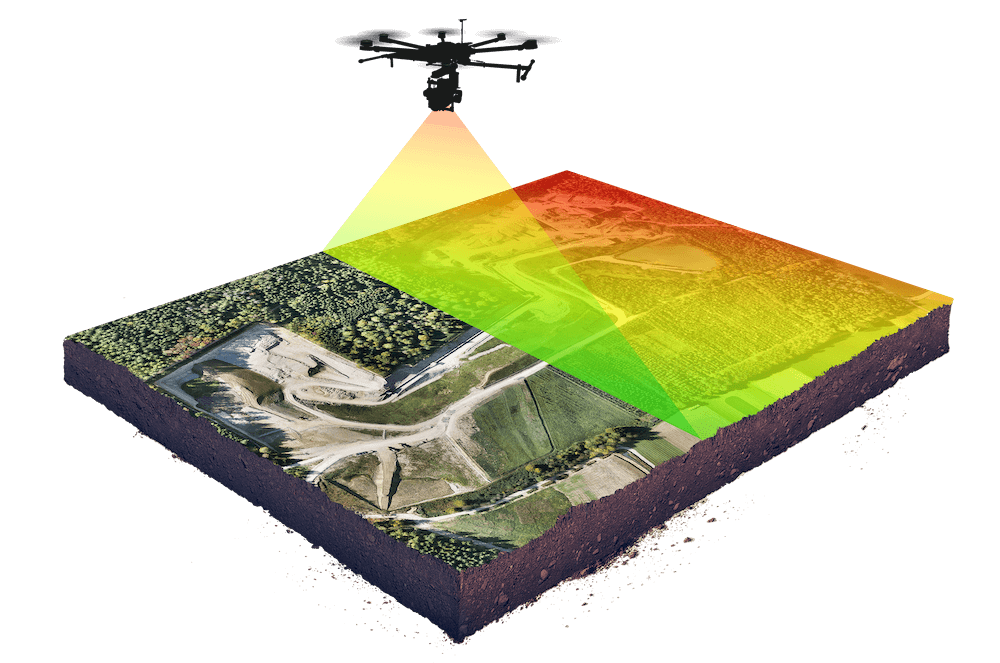
\includegraphics[width=\linewidth]{Images/Related-Work/lidar-drone-example.png}\\
			{(a) UAV usage \URI{https://wingtra.com/drone-photogrammetry-vs-lidar/}}
		\end{minipage}%
		\hspace*{+0.8cm}
		% -----------------
		\begin{minipage}{.47\textwidth}
			\centering
			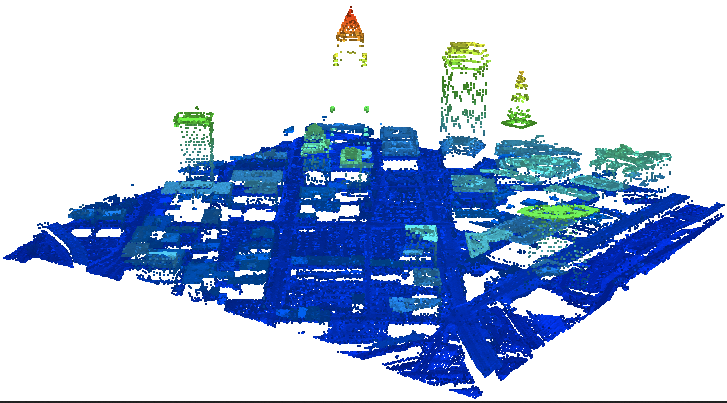
\includegraphics[width=\linewidth]{Images/Related-Work/lidar-cloud.png}\\
			{(b) Cloud Point Data example \URI{https://community.safe.com/s/article/what-is-a-point-cloud-what-is-lidar}}
		\end{minipage}
	% -----------------
    \hfill \break
    \decoRule
	\caption[LiDAR examples]{LiDAR examples}
    \label{fig:drone-lidar}
\end{figure}

Οι συγγραφείς του \cite{lidar-usage-example} κάνουν προσπάθεια χρήσης αυτής της τεχνολογίας, προκειμένου να εξαλείψουν την ανάγκη καμερών - οι οποίες είναι σε άμεση εξάρτηση από τις συνθήκες φωτισμού - ώστε να επιτύχουν ένα long distance drift-free navigation ενός ελικοπτέρου.

Η μεθοδολογία που ακολουθούν είναι να σπάνε το 3D localization problem σε ένα 2D translation problem και ένα 1D altitude problem, τα οποία διαδοχικά προσπαθούν να επιλύσουν. Η γενική αρχή που ακολουθούν είναι ότι προσπαθούν να βρουν την βέλτιστη ευθυγράμμιση μεταξύ των μετρήσεων του \Abbr{LiDAR} και ενός geo-referenced Digital Elevation Model (\Abbr{DEM}) ώστε να καταλήξουν στο 3D world position.

Τα αποτελέσματα που είχαν ήταν final position error της τάξης των 27m σε απόσταση ταξιδιού τα 218km. Χρησιμοποιήθηκαν dataset από ένα Bell 206L (Long-Ranger) helicopter, εξοπλισμένο με ένα Near Earth Autonomy m4 sensor suite το οποίο περιλαμβάνει ένα \Abbr{2D} \Abbr{LiDAR} και ένα fiber-optic \Abbr{IMU}. Ενώ χρησιμοποιήθηκε υπο\-λο\-γι\-στής εξοπλισμένος με quad-core 2.5GHz i7 processor, στον οποίο σε παράλληλο προγραμματισμό έγινε το filtering και matching.

% ---------------------------------------------------------------------------------------------------------
% --------------------------------------------------------------------------------------------------------
\subsection{VSLAM}	\label{sec:related-vslam}
Μία ειδική κατηγορία - με χρήση κάμερας - είναι αυτή στην οποία ακολουθείται η λογική του Visual Simultaneous Localization and Mapping (\Abbr{VSLAM}). Σε αυτήν την περίπτωση, το \Abbr{UAV} προσπαθεί να εντοπίσει τις συντεταγμένες του - αφού πρώτα δημιουργήσει έναν map του χώρου στον οποίο βρίσκεται - ώστε τελικά να βρει την θέση που έχει μέσα σε αυτόν. 
Υπάρχουν διαφορετικοί Simultaneous Lo\-ca\-li\-za\-tion and Mapping (\Abbr{SLAM}) αλγόριθμοι γενικά, με αυτούς που μπορούν να κατηγοριοποιηθούν στους σχετιζόμενος με filtering και αυτούς που σχετίζονται με smoothing τεχνικές \cite{related-slam-difs}. Συνήθως σε αυτούς τους αλγορίθμους, γίνεται εύρεση landmarks στον χώρο, τα οποία χρησιμοποιούνται - \Fig{vslam-drone-visual-perception-example} - στην διαδικασία.

% IMAGE
\FigCaptLabelBasedURL{Images/Related-Work/slam-drone.png}
{VSLAM drone perception example}%
{vslam-drone-visual-perception-example}%
<0.7>%
[vslam-image]%
(https://www.mdpi.com/2504-446X/5/2/41/htm)


Στο \cite{vslam-for-drone-localization} προτείνουν μία αρχιτεκτονική ενός συνεργατικού key-frame-based Multi-\Abbr{UAV} {SLAM} συστήματος. Σε αυτό το σύστημα το κάθε μεμονωμένο drone έχει την δυνατότητα μέσω μίας monocular κάμερας και χρήση real-time Visual Odometry να εκτιμήσει την θέση του, και να παρέχει ένα - περιορισμένων key-frames, εξαιτίας των on-board computation δυνατοτήτων - Local Map του περίγυρου του. Ταυτόχρονα, το σύστημα αποτελείται και από ένα communication module, ώστε τα drone να μπορούν να αλληλεπιδρούν με ένα server, ο οποίος χρησιμοποιείτε για non time-critical computationally expensive processes. 

Βασικές τεχνολογίες που χρησιμοποιήθηκαν ήταν Visual Odometry and Place Re\-co\-gni\-tion βασισμένες στην υλοποίηση του ORB-SLAM2 αλγόριθμου, το \Abbr{ROS} framework για τις επικοινωνίες. Επίσης, ο server που χρησιμοποιήθηκε ήταν ένα Thinkpad T460s notebook εξοπλισμένο με τον τετραπύρηνο Core i7-6600U @ 2.60GHz και 20 GB RAM.

% --------------------------------------------------------------------------------------------------------
% --------------------------------------------------------------------------------------------------------
\subsection{Motion Capture System} \label{sec:related-motion-capturing-systems}
Συχνή χρήση έχουν επίσης τα Motion Capture (\Abbr{MoCap}) Systems \cite{motion-capture}. Όταν αναφερόμαστε σε \Abbr{MoCap} systems, όπως το Vicon \cite{vicon} ή το Optitrack \cite{optitrack}, μιλάμε κυρίως για στατικά, εσωτερικών χώρων συστήματα 
τα οποία είναι υπεύθυνα να ανιχνεύουν και να συλλαμβάνουν την κίνηση σωμάτων. Αποτελούνται από ένα πλήθος καμερών - οι οποίες είναι τοποθετημένες σε προκαθορισμένες θέσεις - μέσω των οποίων μπορεί να εκτιμηθεί η θέση αντικειμένων - όπως drones - στο χώρο αναφοράς. Παράδειγμα αυτού υπάρχει στο \Fig{motion-capturing-drone-swarm}

% IMAGE
\FigCaptLabelBasedURL{Images/Related-Work/optitrack.png}%
{Optitrack Motion Capturing System for drone swarm localization}%
{motion-capturing-drone-swarm}%
<0.6>%
(https://optitrack.com/systems/)

Στην προσπάθεια τους οι \cite{related-motion-captu} χρησιμοποιούν ένα τέτοιο \Abbr{MoCap} system, προκειμένου να δημιουργήσουν ένα multi-\Abbr{UAV} αλγόριθμο ελέγχου για centralized formation flight. 

Στα πειράματα τους χρησιμοποιήθηκαν το Vicon, ως drone τα Parrot AR Drone 2.0, ενώ η υλοποίηση έγινε στο περιβάλλον του MATLAB/SI\-MU\-LI\-NK αξιοποιώντας το AR Drone Simulink Development Kit.
